% ABLS - term-long paper
% Christopher Wood

\documentclass{sig-alternate}

\usepackage{url}
\usepackage{color}
\usepackage{enumerate}
\usepackage{balance}
\usepackage{verbatim}
\usepackage{enumitem}
\usepackage[table]{xcolor}
\usepackage{multicol,multirow}
\usepackage{subfig}
\usepackage{dcolumn}
\usepackage{palatino}
\usepackage{bbm}
\usepackage{url}
\usepackage{verbatim}
\usepackage{algorithm}
\usepackage[noend]{algorithmic}
\usepackage{fancybox, fancyvrb}
\usepackage{listings}
\usepackage{amsmath}
\usepackage{array}
\usepackage{mathtools}

\newenvironment{definition}[1][Definition]{\begin{trivlist}
\item[\hskip \labelsep {\bfseries #1}]}{\end{trivlist}}

\permission{}
\CopyrightYear{2012}
%\crdata{0-00000-00-0/00/00}
\begin{document}

\title{ABLS: A Secure Logging System with Attribute-Based Log Access and Automated Auditing in the Cloud}
\numberofauthors{1}
\author{
\alignauthor{
Christopher A. Wood \\
Department of Computer Science \\
{\tt caw4567@rit.edu}
}}
\date{\today}
\maketitle
\begin{abstract}
User-based non-repudiation is an increasingly important property of cloud-based applications. It provides irrefutable 
evidence that ties system behavior to specific users, thus enabling strict enforcement of organizational security policies. 
System logs are typically used as the basis for this property. Thus, the effectiveness of system audits based on log files 
reduces to the problem of maintaining the integrity and confidentiality of log files without sacrificing the usefulness
of the data in these log files. Furthermore, since useful log messages may contain sensitive information, 
access control for log 
data should be implemented so as to restrict access to only those parties that need to view it (i.e. generating users,
colleagues of generating users, auditors, system administrators, etc). ABAC has been a common technique used to
satisfy this requirement. 
In an ideal setting, automated audits on encrypted log data would also be possible so as to support manual
inspections done to comply with federal regulations or compliance laws.

In this work we address all of the aforementioned issues with a proof-of-concept system called ABLS, an attribute-based logging system designed
to support automated audits of encrypted log data based on user-defined security policies. Confidentiality of and access to
sensitive log information is enforced using ciphertext-policy attribute-based encryption (CP-ABE) with a minimal number
of log-related roles, and thus a small number of attributes, to avoid the problem of increasing encryption computational
complexity with attribute explosion. The integrity of log data is guaranteed using forward-secure hash-chain constructions of log chains. In this paper we present the preliminary design of ABLS and discuss how audit trails are 
constructed from log data using the aforementioned confidentiality and integrity techniques, automated audit tasks are defined and specified, and how the system may be used in practical applications.
\end{abstract}

\section{Introduction}
User-based non-repudiation is a security property that provides indisputable evidence linking
system behavior to individual users. Cryptographically speaking, 
non-repudiation requires that the integrity and 
origin of all data should be undeniable and provable. In essence, this enables system audits to be conducted that can
identify data misuse, and thus, potential security policy violations, by comparing the contextual information 
of system events (e.g. source user, time of the event, etc) with all entities authorized to invoke such events. 
Therefore, treating non-repudiation as a required system quality attribute in the architecture is likely to 
become a common trend in the commercial, government, and even more specifically, the health-care domain.

Audits typically use log files to determine the ``who, what, when, and how'' of events that take 
place during a system's lifetime. In order to provide accurate information for non-repudiation purposes,
it is often necessary to place some amount user-sensitive data in these log files that can be used
to trace data back to its origin. As such, logs of events generated by a client that is being served must
maintain data confidentiality and integrity should the system be compromised. Historical approaches
to the problem of log security are based on tamper-resistant hardware and maintaining continuous 
secure communication channels between a log aggregator and end user \cite{Schneier1999-Secure}. 
However, such solutions are not applicable in the context of cloud-based applications. 

Recent approaches have relied on combinations of encryption and signature techniques \cite{Ma2008-FssAgg}. 
Symmetric-key and public-key encryption of log entries are very common confidentiality techniques 
proposed in the literature. Unfortunately, these schemes are becoming less useful in modern corporate environments with
dynamically changing users and access policies.
There is a need for robust access control mechanisms that enable dynamic user addition and revocation
with minimal overhead. In other words, continuously re-encrypting a subset of the log database should be avoided. 
Both symmetric- and public-key cryptosystems suffer in that access policies must be tied directly to keys used for
encryption and decryption. If the access policy for a set of log messages needs to be changed, then both the keys used to
encrypt and decrypt such log entries will need to be regenerated and distributed, and the entries must also
be re-encrypted. Both of these tasks can be very expensive. 

In addition, symmetric-key cryptosystems require keys to be shared among users who need access to the 
same set of logs. This requires a secure and comprehensive key management and distribution scheme and
supporting policy. In a similar vein, public-key cryptosystems (e.g. RSA and ElGamal) suffer 
from the extra data transfer and storage requirements for large cryptographic keys and certificates. 
In some systems there may be insufficient resources to maintain a public-key infrastructure (PKI) for managing 
keys and digital certificates for all users. 

In terms of log file integrity, aggregate signature schemes that support forward secrecy through the use of 
symmetric- and public-key cryptosystems are very popular solutions in the literature \cite{Yavuz2009-BAF}.
However, while symmetric-key schemes promote high computational efficiency for signature generation, but they 
do not directly support public verifiability for administrators and auditors. This means that robust key 
distribution schemes or the introduction of a trusted third party (TTP) are needed to ensure that all 
required parties can verify the necessary log data. Such schemes also 
suffer from relatively high storage requirements and communication overhead. Public-key 
schemes have similar issues, as the increased key size leads to even larger storage 
requirements and less computational efficiency. Also, public-key schemes introduce the need
for a trusted certificate authority to grant certificates for all parties that sign log information. % TODO: find a citation for this...
One time-tested technique for supporting log file integrity is the use of authenticated 
hash-chains \cite{Schneier1999-Secure}, which will be a focus of this paper.

Collectively, we see that a balance between encryption and signature generation and verification performance is
needed to support the unique scalability and resource usage requirements for cloud-based applications.
Furthermore, the selected cryptographic primitives to encrypt, sign, and verify data must not exacerbate the
problem of dynamically changing access control policies and user privileges. Role-based Access Control (RBAC),
which first gained popularity in the mid 1990s \cite{Sandhu1996-RBAC} \cite{David1992-RBAC} and was later 
proposed as a standard for the National Institute of Standards and Technology in 2001\cite{Ferraiolo2001-RBAC}, 
is an increasingly popular access control policy that enables users to be associated with roles that change
less frequently. In the context of maintaining the confidentiality of log messages generated by many users,
RBAC surpasses traditional mandatory and discretionary access control (MAC and DAC) 
\cite{Abrams1990-AccessControl}.

More recently, attribute-based access control (ABAC) \cite{shen2006attribute} \cite{alipour2011policy} 
\cite{zhu2008attribute} has been developed to provide more fine-grained access control to sensitive data. 
It is common practice to specify user roles as attributes
in this access control scheme, thus enabling the benefits of RBAC with fine-grained access control.
Attribute-based encryption (ABE) \cite{Goyal2006-ABAC}, a new cryptographic primitive that uses 
user attributes (or roles, in this context) to maintain the confidentiality of user-sensitive data, has an appealing application
to logging systems maintained in the cloud and is capable of satisfying the aforementioned confidentiality 
requirements. 

In this paper we address all of the aforementioned issues with a proof-of-concept system called ABLS, 
an attribute-based logging system designed
to support automated audits of encrypted audit trails (log data) based on user-defined security policies. Access to
sensitive log information is enforced using ciphertext-policy attribute-based encryption (CP-ABE) 
\cite{Bethencourt2007-CPABE} with a minimal number
of log-related roles, and thus a small number of attributes, to avoid the problem of increasing encryption computational
complexity with attribute explosion. We present the initial design of ABLS and discuss how audit trails are 
constructed from log data to ensure confidentiality and integrity, the design through which automated audit tasks are 
defined and specified, a preliminary analysis of the performance and storage overhead incurred by the system, and, finally,  
how the system may be used in practical applications.

%The paper is organized in a top-down fashion, starting with the structure of log data and corresponding ability
%to define automated audit tasks. Using this foundation, we then introduce the relational data model used to persist
%log information, followed by the cryptographic access control mechanisms used to maintain the confidentiality
%of log data and audit trails. Finally, we conclude with a practical use case for ABLS in the context of healthcare 
%organizations.

\section{Secure Logging Requirements}
The most fundamental requirements for a secure logging system are that it provides log data integrity
and confidentiality. In the context of a secure logging system, integrity is based on the forward-secure
stream integrity model \cite{Bellare1997-ForwardIntegrity}, which guarantees that log data cannot be forged or rearranged 
within the stream of log messages and that the logging system is resilient against attacks that try to recover old keys after a 
machine has been compromised (hence, forward-secure).

Research into this problem has since revealed that a variety of other realistic
requirements also exist, including a resilience to truncation and delayed detection attacks, 
minimal reliance on an online server for log storage and verification, and storage efficiency. 
For completeness, truncation and delayed detection attacks are defined below, based on 
explanations presented in \cite{ma2008practical}. These attacks assume the presence of an untrusted
log server $\mathcal{L}$ and a trusted machine $\mathcal{T}$.

\begin{itemize}
  \item \textbf{Truncation attack} - An attack in which a set of log entries residing on an untrusted log
servers is truncated, or shortened so as to remove suspicious events, without being detected by 
synchronization with the trusted log server.
  \item \textbf{Delayed detection} - An attack in which log entries on an untrusted log server $\mathcal{L}$ can be 
  modified by an attacker who possesses the authentication key $A_i$ after compromising the system between
  log entries $L_i$ and $L_{i+1}$. With this key, the attacker can easily change new entries in the log. However, once the trusted machine $\mathcal{T}$ synchronizes with $\mathcal{L}$ to check the integrity of the log messages, this attack is immediately detected. Of course, significant damage and log data modification could have already been done during this time window (i.e. between the time when $\mathcal{L}$ was compromised and when it was synchronized with $\mathcal{T}$).
\end{itemize}

%\section{Cryptographic Primitives}
%This scheme 
%TODO: introduce CP-ABE and FssAgg primitives, and how they're used for confidentiality and integrity, respectively

\section{Log File Reliability}
\label{sec:LogConstruction}

%In this section we present our log generation and verification schemes.
%They are influenced by past work done by Schneier et al ,
%Bellare et al. \cite{Bellare1997-ForwardIntegrity}, Ma et al. \cite{Ma2008-FssAgg},
%and Yavuz et al. \cite{Yavuz2009-BAF}. 

Log file reliability, which reduces to log integrity, is achieved through hash chains and 
message-authentication codes (MACs), which is a technique first introduced by Schneier et al 
\cite{Schneier1999-Secure} and motivated by Bellare et al \cite{Bellare1997-ForwardIntegrity}. 
Each log entry is a five-tuple element that contains the generating source
information (i.e. the user $U$ and session identifier $S$), the encrypted payload $C$ of the log data $D$, a 
hash digest $X$ that provides a link between the current and previous hash chain entries, and an 
authentication tag $Y$ for the digest $X$. Formally, each log entry $L_i$ is built using the following definitions:
\begin{align*}
X_i = & H(X_{i - 1}, E_{PK}(D_i)) \\ % rationale: need to link this entry to previous for chaining
Y_i = & HMAC_{A_i}(X_i) \\ 
L_i = & (U_{i}, S_{i}, E_{PK}(D_i), X_i, Y_i) % rationale for u/s: searhability
\end{align*}

%\begin{figure*}[ht!]
%  \centering
%  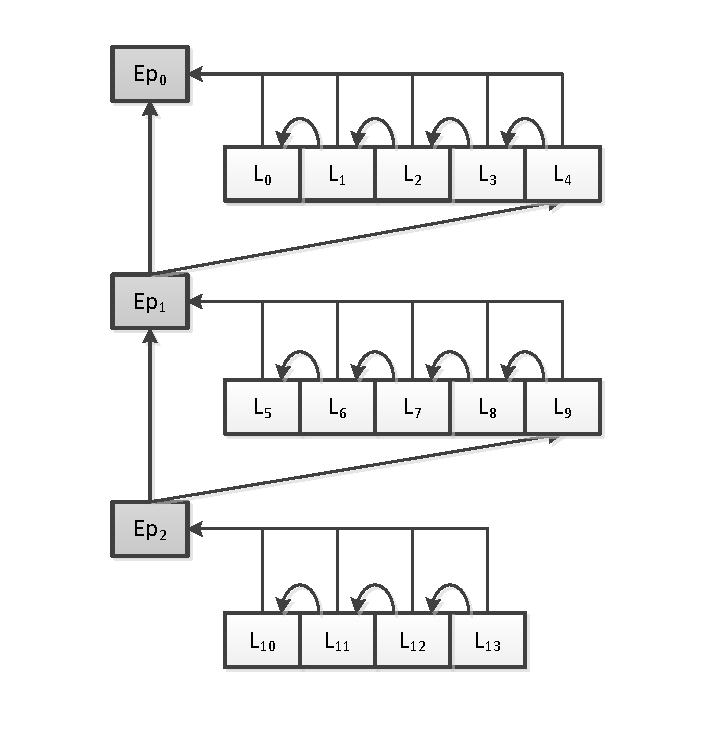
\includegraphics[scale=0.8]{images/hashchain.pdf} \\
%\caption{A visual depiction of the hash chain construction scheme. In this case, the epoch window is $5$ log entries, as shown by the epoch
%cycle after $5$ consecutive log entries.}
%\label{fig:hashChain}
%\end{figure*}

In this scheme the $X_i$ elements are used to link together consecutive entries in 
the hash chain. Similarly, the $Y_i$ elements are used to provide authentication 
for the $X_i$ element as an authentication tag. Also, the elements $PK$ and $A_i$
are the policy key (which is discussed later) and MAC key for this hash chain. The 
initial value for the MAC key $A_0$ is randomly generated when a user session is 
created, and is continually evolved every time it is used with a forward-secure
pseudorandom function $H$ as follows:
\begin{align*}
A_{i+1} = H(A_i)
\end{align*}
In order to prevent truncation and deletion attacks, a single entity $T_i$ for the entire log 
chain is updated as the log chain is iteratively constructed. Formally, $T_i$ is
computed as follows:
\begin{align*}
T_i = & HMAC_{B_i}(L_{i}, T_{i - 1}) \\
T_0 = & HMAC_{B_0}(L_{i}, 1)
\end{align*}
$B_0$ is a secret key that that is randomly generated when the log chain for a user session
is initialized. Similar to the key $A_i$, this key is evolved with a forward-secure pseudorandom function 
$H$ as follows:
\begin{align*}
B_{i+1} = H(B_i)
\end{align*}
This entity creation and hash chaining scheme could be replaced with a publicly-verifiable Forward Secure 
Sequential Aggregate (FssAgg) signature scheme backed by a trusted certificate authority (CA) to support 
forward-secure stream integrity. However, since we do not assume the presence of such a CA, we did
not make this modification to our logging scheme. We refer the reader to \cite{Ma2008-FssAgg} for a more thorough treatment of FssAgg aggregate signature schemes and their role in updating the single log chain entity. 

%A visual representation of this protocol is shown in Figure \ref{fig:tagChain}. It is
%important to note that a chain of $T_i$ elements is not maintained. Instead, only the
%most recent element is persisted to the database. This is critical to prevent
%truncation attacks.

%\begin{figure*}[ht!]
%  \centering
%  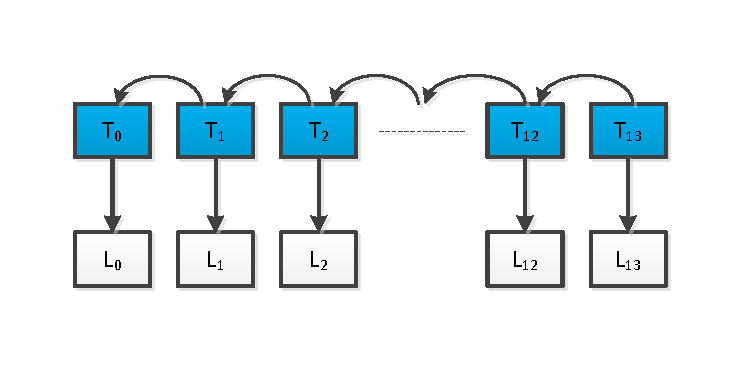
\includegraphics[scale=0.8]{images/tagchain.pdf} \\
%\caption{A visual depiction of the protocol used to build the log chain authentication tag.}
%\label{fig:tagChain}
%\end{figure*}

\subsection{Verification Modes}
\label{log:VerificationModes}

The ABLS log construction scheme enables two different modes of verification to be implemented,
each of which has different integrity and performance guarantees. The first mode of verification
requires any entity, trusted or untrusted, to walk the log chain, computing the digest $X_i$ and comparing it to the value
stored in the database. However, this method does not guarantee the integrity of the log chain because
an attacker may easily modify the $X_i$ values of the hash chain if they compromise the log server.

The second mode of verification requires a trusted verifier task $\mathcal{V}$ to use the initial
hash chain key $A_0$ and entity key $B_0$ to walk the log entries, computing both $X_i$ and $Y_i$,
and comparing them against the values stored in the database. At the end of a traversal of a hash chain of length $n$,
$\mathcal{V}$ will compare the final entity value $B_n$ against the value stored in the database and only accept
the hash chain if these values are equal. While this mode does not lend itself
to public verifiability, it guarantees the integrity of the log chain if a forward-secure MAC is used 
and the keys $A_0$ and $B_0$ are protected.

\section{Log Access Control}
Access control for all of the log data is enforced using ciphertext policy attribute-based encryption 
(CP-ABE), a new pairing-based cryptographic primitive that embeds complex
access policies in ciphertext which specify the secret keys that can be used for decryption \cite{Bethencourt2007-CPABE}. 
In CP-ABE, secret keys are analogous to sets of attributes, and access policies are defined using 
tree-like access structures of logical AND and OR gates, where each leaf in the tree is an attribute. Implementations of 
CP-ABE schemes are usually based on the construction of a bilinear mapping between two elliptic curve 
groups \cite{Bethencourt2007-CPABE} \cite{Junod2010-ABE}. For completeness, we define both of these terms below.

\begin{definition}
Let $\mathbb{F}_p$ be a finite field where $p > 3$ is a prime, and $a, b \in \mathbb{F}_p$ such that
\begin{align*}
4a^3 + 27b^2 \not= 0 \mod p \in \mathbb{F}_p
\end{align*}

An \emph{ellptic curve} $E[\mathbb{F}_p]$ is the set of solutions $(x, y)$ to the equation
\begin{align*}
y^2 = x^3 + ax + b \mod p \in \mathbb{F}_p[x],
\end{align*}
together with the point at infinite $0$.
\end{definition}

\begin{definition}
Let $G_1$ and $G_2$ be cyclic groups of prime order $p$ and $g$ a generator of $G_1$. We say that $e$ is a \emph{bilinear map} defined as $e : G_1 \times G_2$, where $|G_1| = |G_2| = p$. This bilinear map satisfies the following properties:
\begin{itemize}
	\item Bilinearity: For all $u, v \in G_0$ and $a, b \in \mathbb{Z}_p$, we have $e(u^a, v^b) = e(u,v)^{ab}$
	\item Non-degeneracy: $e(g, g,) \not= 1$
	\item Computability: Both $G_1$ and $G_2$ are efficiently computable
\end{itemize}
\end{definition}

In the original construction of the CP-ABE scheme, Bethencourt et al \cite{Bethencourt2007-CPABE} defined five different procedures 
used in the cryptosystem: \emph{Setup}, \emph{Encrypt}, \emph{KeyGeneration}, \emph{Derypt}, and 
\emph{Delegate}. For completeness, we define each of these procedures below:
\begin{itemize}
	\item \textbf{Setup} - This procedure takes the implicit security parameter as input and outputs the public and master keys $PK$ and $MK$.
	\item \textbf{Encrypt}(\textbf{PK}, M, $\mathbb{A}$) - This procedure will encrypt $M$, a plaintext message, to produce a ciphertext $CT$ such that only a user that possesses a set of attributes that satisfies the access structure $\mathbb{A}$ will be able to decrypt the message. The encryption process embeds $\mathbb{A}$ into the ciphertext.
	\item \textbf{KeyGeneration}(\textbf{MK}, $\mathbb{S}$) - This procedure generates a private key $SK$ using the master key $MK$ and set of attributes $S$ that describe the private key. 
	\item \textbf{Decrypt}(\textbf{PK}, \textbf{CT}, \textbf{SK}) - This procedure decrypts the ciphertext $CT$ using the provided secret key $SK$ to return the original message $M$. Decryption is only successful if the set $S$ of attributes, which is associated with the key $SK$, satisfies the access policy embedded within the ciphertext (which is part of the access structure $\mathbb{A}$).
	\item \textbf{Delegate}(\textbf{SK}, \~{S}) - This procedure outputs a secret key \~{$SK$} for the set of attributes \~{$S$}, where \~{$S$} $\subset S$, the set of attributes associated with the secret key \textbf{SK}.
\end{itemize}

\subsection{Access Policy Definition}

A major component of ABLS is the policy engine, which maps access policies defined on an individual event basis to 
the corresponding access tree used for encryption. For example, an access policy might state that only User
XYZ, or physician assistants or nurse practitioners from Medical Group A, are allowed to access data associated
with an event $E$. The corresponding access tree for this policy is shown in Figure \ref{fig:accessTree}.  

\begin{figure}[ht!]
\begin{center}
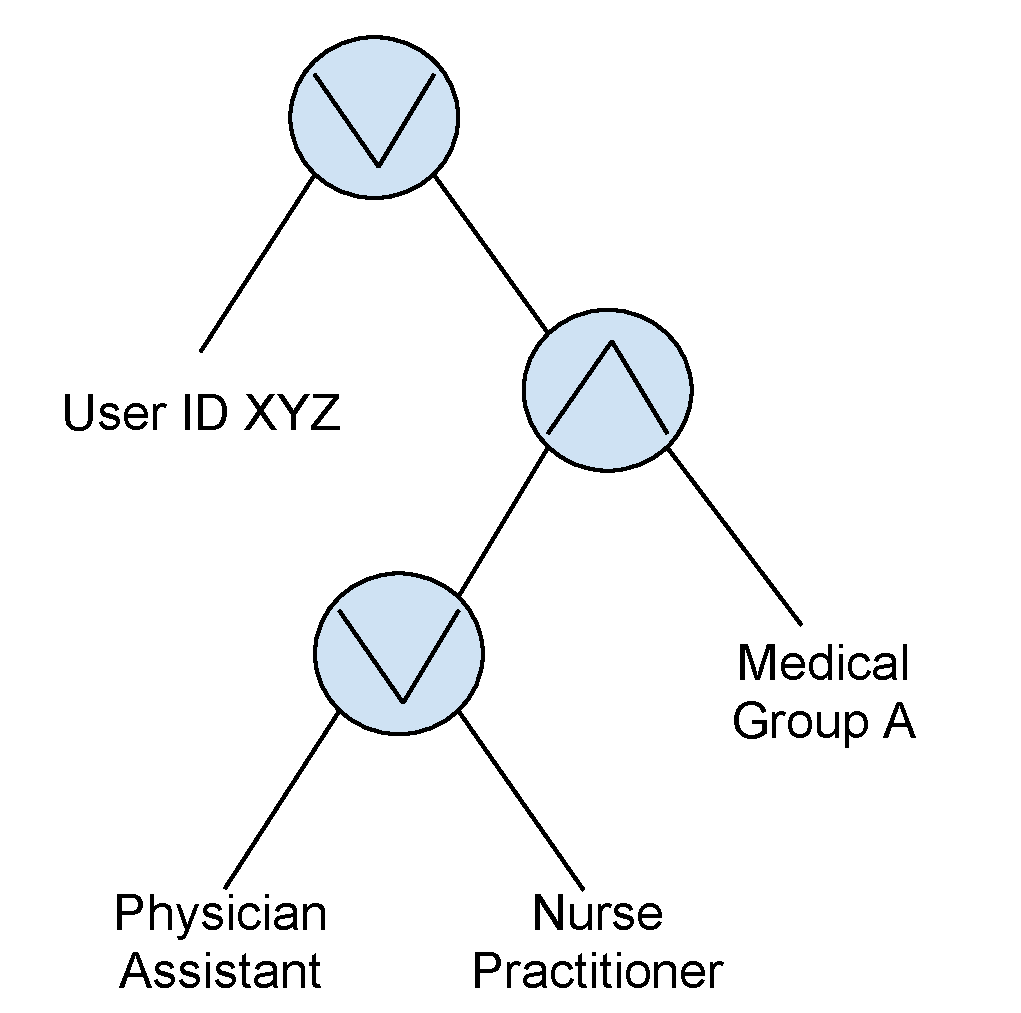
\includegraphics[width=1.5in]{images/cpabePolicy.pdf}
\caption{Access tree for a policy that only enables access to user XYZ, Medical Group A physician assistants, and Medical Group A nurse practitioners.}
\label{fig:accessTree}
\end{center}
\end{figure}

ABLS is unique in that temporal attributes can be embedded in the access policy trees. For example, an attribute
that states the requesting user is a ``colleague of User XYZ'' can be added to the access policy. As will be discussed 
in the next section, the addition of this type of temporal, or context-sensitive, attribute enables flexible addition and 
revocation of access from users who do not own log data. 

Our logging scheme makes the assumption that events, and the access policies for all data associated
with such events, are well defined, which is often the case with organizations that must
comply with federal regulations like HIPAA \cite{annas2003hipaa}. With this
assumption, the behavior of the policy engine in generating access policies is dependent on
administrator-defined policy rules for events of interest and the corresponding attributes of
system users and data that trigger such events. In this way, policy rules are coupled to events so that 
policies for access are generated based on the type of event that occurred and the user who is requesting 
access to such information. System administrators may define these policies using the standard eXtensible
Access Control Markup Language \cite{anderson2005comparison}. While the current version of ABLS does not
support the ability to parse such XACML documents for specifying event encryption policies, this is an avenue of
work that we hope to explore in the future.

\subsection{Key Generation and Management}
Pairing-based cryptography is computationally expensive, and under the assumption that ABLS might be subject 
to very heavy traffic loads at any particular time, the 
overhead of encrypting data to be stored in the database should be as minimal as possible. Therefore, each unique
policy that is needed to encrypt a log message is associated with a randomly-generated symmetric policy 
key $PK$, which is in turn encrypted using CP-ABE and then serialized to be stored in the key database. 
This design enhancement enables increased throughput without sacrificing the 
level of confidentiality granularity that is needed for each log entry. However, should an 
unencrypted policy key for a given user's session become compromised, the remaining entries in the 
log database that share the same key $PK$ are at risk of being compromised. 

The basic procedure for encrypting a log entry is shown in Algorithm \ref{alg:encrypt}. Once encrypted, the ciphertext
is stored in the database with the rest of the information necessary to continue the log chain for a given user's session.
  
\begin{algorithm}[h] %[htb]
\caption{Log entry encryption} \label{alg:encrypt}
\begin{algorithmic}[1]
\REQUIRE{An unencrypted piece of log data $D_i$ for session $S_j$ of user $U_k$}
% \ENSURE{The number of all minimum $(s,t)$-cuts of $G$}

% I decided not to list the input/output in this case, so that's why the above two lines are commented out
\STATE{Let $P$ be the access control policy for the data $D_i$, as determined by the policy engine}
\IF{The symmetric key $PK$ for $(U_k, S_j)$ has not been generated for $P$}
  \STATE{Randomly generate $PK$ and encrypt it with the CP-ABE encryption module using $P$, yielding $K_E$}
  \STATE{Persist $K_E$ to the key database}
\ELSE
  \STATE{Query the database for $K_E$, the encrypted key for policy $P$.}
  \STATE{Decrypt $K_E$ using the attributes of user $U_k$, yielding $PK$}
\ENDIF
\STATE{Encrypt $D_i$ with $PK$, yielding $E_{PK}(D_i)$}
\STATE{Persist $E_{PK}(D_i)$ to the log database}
\end{algorithmic}
\end{algorithm}

In order to improve the performance of the logger, the per-policy symmetric keys used for encryption for a 
user session are kept in memory until the session has been closed. This avoids the need for the logger 
to query the database for the key when a new piece of log data arrives. 

By default, the secret keys used for decryption are never cached in the system's local memory. Since it is
expected that log entries will be read much less frequently than they will be written, such keys are generated
on demand by querying the appropriate database. Furthermore, the key generation process can be done in two ways. 
For policy rules that limit the access to only the generating user, only a single query to the attribute database
is required to establish the user's secret key and then decrypt the data for all log entries corresponding to that rule. 
With this key the user may decrypt these entries offline without the need to query the policy engine for the 
appropriate access rights.

Conversely, for access policy rules that embed temporal or context-sensitive attributes (i.e. attributes for colleagues or other 
users related to the source user), the policy engine must first query the system database to ensure the requesting 
user meets the relationship criteria set in place by the policy. Then,
if this is successful, the policy engine will grant the appropriate secret key to the requesting user. The tradeoff
is that, while an online TTP is needed for such colleagues to access the log entry contents, it is significantly easier
for the system administrators to manage who has access to specific log entries aside from the original source user.
Simply modifying relationships in the system database is sufficient to revoke access from certain users.

In order to maintain the security of the system at runtime, it is necessary to cycle the master and public keys
associated with the CP-ABE encryption scheme. Our current system does not support this feature, but there are two
ways that it could be implemented. The first way is to persist the old master and 
public keys to a safe location that could be obtained by audit and verification tasks if needed. The second way is 
to re-encrypt the entire log database with the new master and public key. Unfortunately, this would not only require the system to be 
brought offline during the update (in order to avoid synchronization issues with live traffic), but it would also
mean that the new master and public key serve as a single point of failure for the entire database if compromised. 
Therefore, future versions of this system will to implement the former approach to manage keys. It would be
best to determine the key cycle lifetime based on empirical data associated with the growth of the log database.
Intuitively, in order to maintain auditing and verification efficiency, the cycle frequency should be defined as 
a monotonically increasing function that is proportional to the growth of the database. 

\section{Structured Log Data for Automated Audits}
Current technological solutions for automated audits in organizations where the usage of audit trails is required for compliance activities
are considered to be ineffective \cite{president2004revolutionizing}. In order to support automated audits of audit trails,
it is necessary to specify a formal structure for this data that matches organizational security policies. 
Therefore, a major motivating factor for the ABLS log data structure is that it can be mapped to and from 
realistic security policies. In this context, we make
the assumption that a security policy can be stated as a set of \emph{negative requirements}. For example, in 
the healthcare domain, one 
such requirement might be that a doctor is not allowed to change their patient's address. In order to conduct an 
automated audit for violations of this policy, we first translate this semantically-rich requirement into a language
whose structure can be easily mapped to a relational data model. This enables us to leverage the power of 
structured query languages (i.e. SQL) to automatically search for policy violations.

One solution for parsing security policy requirements into relational data is to define a grammar for producing 
requirement strings. Using the NIST RBAC model of access control as motivation \cite{Ferraiolo2001-RBAC}, 
we specify the set of terminals and relations in the grammar to 
be the set identifiers USER, OBS, and OPS. These finite sets are minimal enough to 
allow the specification of most security policies, thus making it suitable for our needs. 

LAudit, a \emph{simple} context-free grammar with only a single non-terminal and the aforementioned terminals, is shown below.\\

{\setlength\tabcolsep{4pt}
\begin{tabular}{>{$}l<{$}>{$}r<{$}>{$}l<{$}}
  \text{LAudit} &\Coloneqq & \text{USER OPS}\\
  &| & \text{USER OPS OBS} \\
  &| & \text{USER OPS OBS USER} \\
\end{tabular}}
\vspace{.35cm} 

In this context, USER, OPS, and OBS are all finite sets composed of the users, operations, and objects of a
system, as specified by the NIST RBAC model \cite{Sandhu2000-nist-rbac}. While simple, this language effectively
captures the source of log events (i.e. the ``who'') and the affected elements and system objects of these events (i.e. the ``what''). ABLS is capable of appending a timestamp to every that it receives, which covers the time-specific information for an event (i.e. the ``when''). 

ABLS clients must submit log messages according to a pre-defined schema that captures
all of the information in LAudit. A simple JSON schema that can be used for constructing log messages 
is shown below.

\begin{lstlisting}
[
    {
        user : int,
        session : int,
        action : int (or String),
        object : int (or String),
        affectedUsers : [int]
    }
]
\end{lstlisting}

\section{Relational Model and Privacy Implications}
\label{sec:model}
In order to capture the audit information in a relational model to enable efficient and automated queries, 
the events, actions, objects, and affected users are all coupled to the incoming log data. The resulting relational
model is shown in Figure \ref{fig:schema}.

This schema only corresponds to the log database in ABLS. There are in fact four databases altogether that must be maintained by ABLS:
the log, key, user, and policy database. The log database maintains all information in the 
log chain and associated events for every 
single user and session pair. The key database stores the cryptographic keys that were used to construct
such log chains. The user, and policy databases store user information and policy rules for ABLS, respectively. 

In order to link the entries in the log tables to their corresponding verification and encryption keys in the key database,
common user and session IDs are used (though not as the primary key for the tables since they do not satisfy
the uniqueness property). However, storing user and session information in plaintext may lead to a privacy violation
if the database is compromised. Therefore, using a technique inspired by the ``onion encryption'' design in
CryptDB \cite{Popa2012-CryptDB}, this information is now deterministically encrypted before being stored in the database.

This procedure works by encrypting the user and session attributes with a symmetric key generated
from the logger's master key $M_k$ salted by the target table identifier. In mathematical
terms, the encrypted user and session IDs, $[U_i]$ and $[S_j]$, stored in table $T$ are generated as follows.
\begin{align*}
[U_i] = E(M_k || H(T), U_i) \\
[S_j] = E(M_k || H(T), S_j) \\
\end{align*}
Using the table identifier as a salt to the master key 
enable ensures that tables do not share any common information about the user, which helps prevent against 
inference attacks in the event that the database servers are compromised. Furthermore, this enables verifiers,
who will have access to $M_k$ through the key manager, to decrypt log entries and recover the user identifier 
so that they may check the contents of the other databases as needed.

In the log data model, all Action and Object records are stored in plaintext. These tables store elements of a finite set, so
encrypting them would not derail a determined attacker. However, all information about affected users is encrypted 
(masked) using the previously mentioned encryption technique. As such, an attacker can infer
information about what types of objects were operated upon, but they cannot determine the specifics of these actions
or the users who performed them without compromising the master key $M_k$. We feel as though this strikes
a good balance between robust audit specification, reasonable measures of audit and log efficiency, user privacy, and log security. 

\begin{figure*}[htb!]
\begin{center}
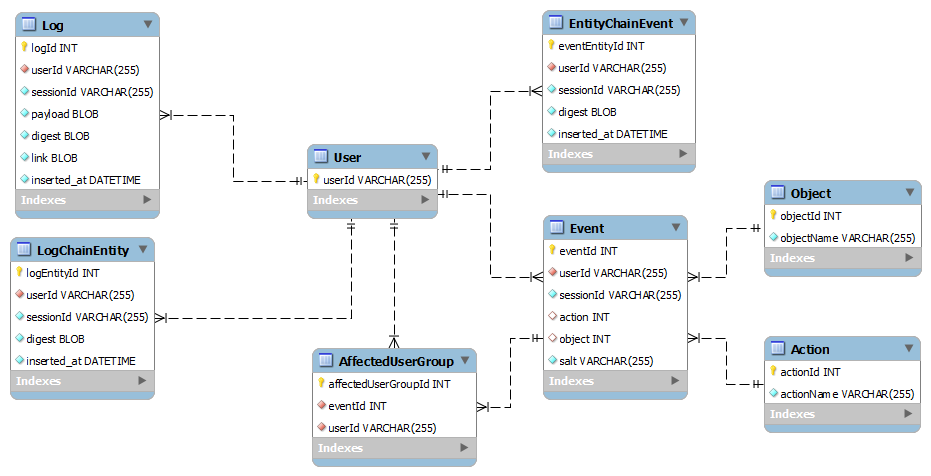
\includegraphics[width=5in]{images/logSchema.png}
\caption{ER diagram depicting the relational schema for the log data model.}
\label{fig:schema}
\end{center}
\end{figure*}

\section{ABLS System Architecture}
\label{sec:deployment}
ABLS is designed to be a centralized logging system backed by a set of distributed databases. A major
goal for the architecture was horizontal scalability, which is achieved through separation of the log and 
audit consumption and production processes. Message queues are used to collate all data to be processed
by an ABLS instance from an arbitrary number of clients, which means that the only bottleneck in the system is how
fast these messages can be served by the ABLS instance. If deployed in the cloud (e.g. Amazon AWS), ABLS can 
be granted a large enough worker thread pool to optimize log and audit message processing. A graphical context
diagram for the ABLS system architecture that highlights these design elements is shown in Figure \ref{fig:deployment}.

\begin{figure*}[htb!]
\begin{center}
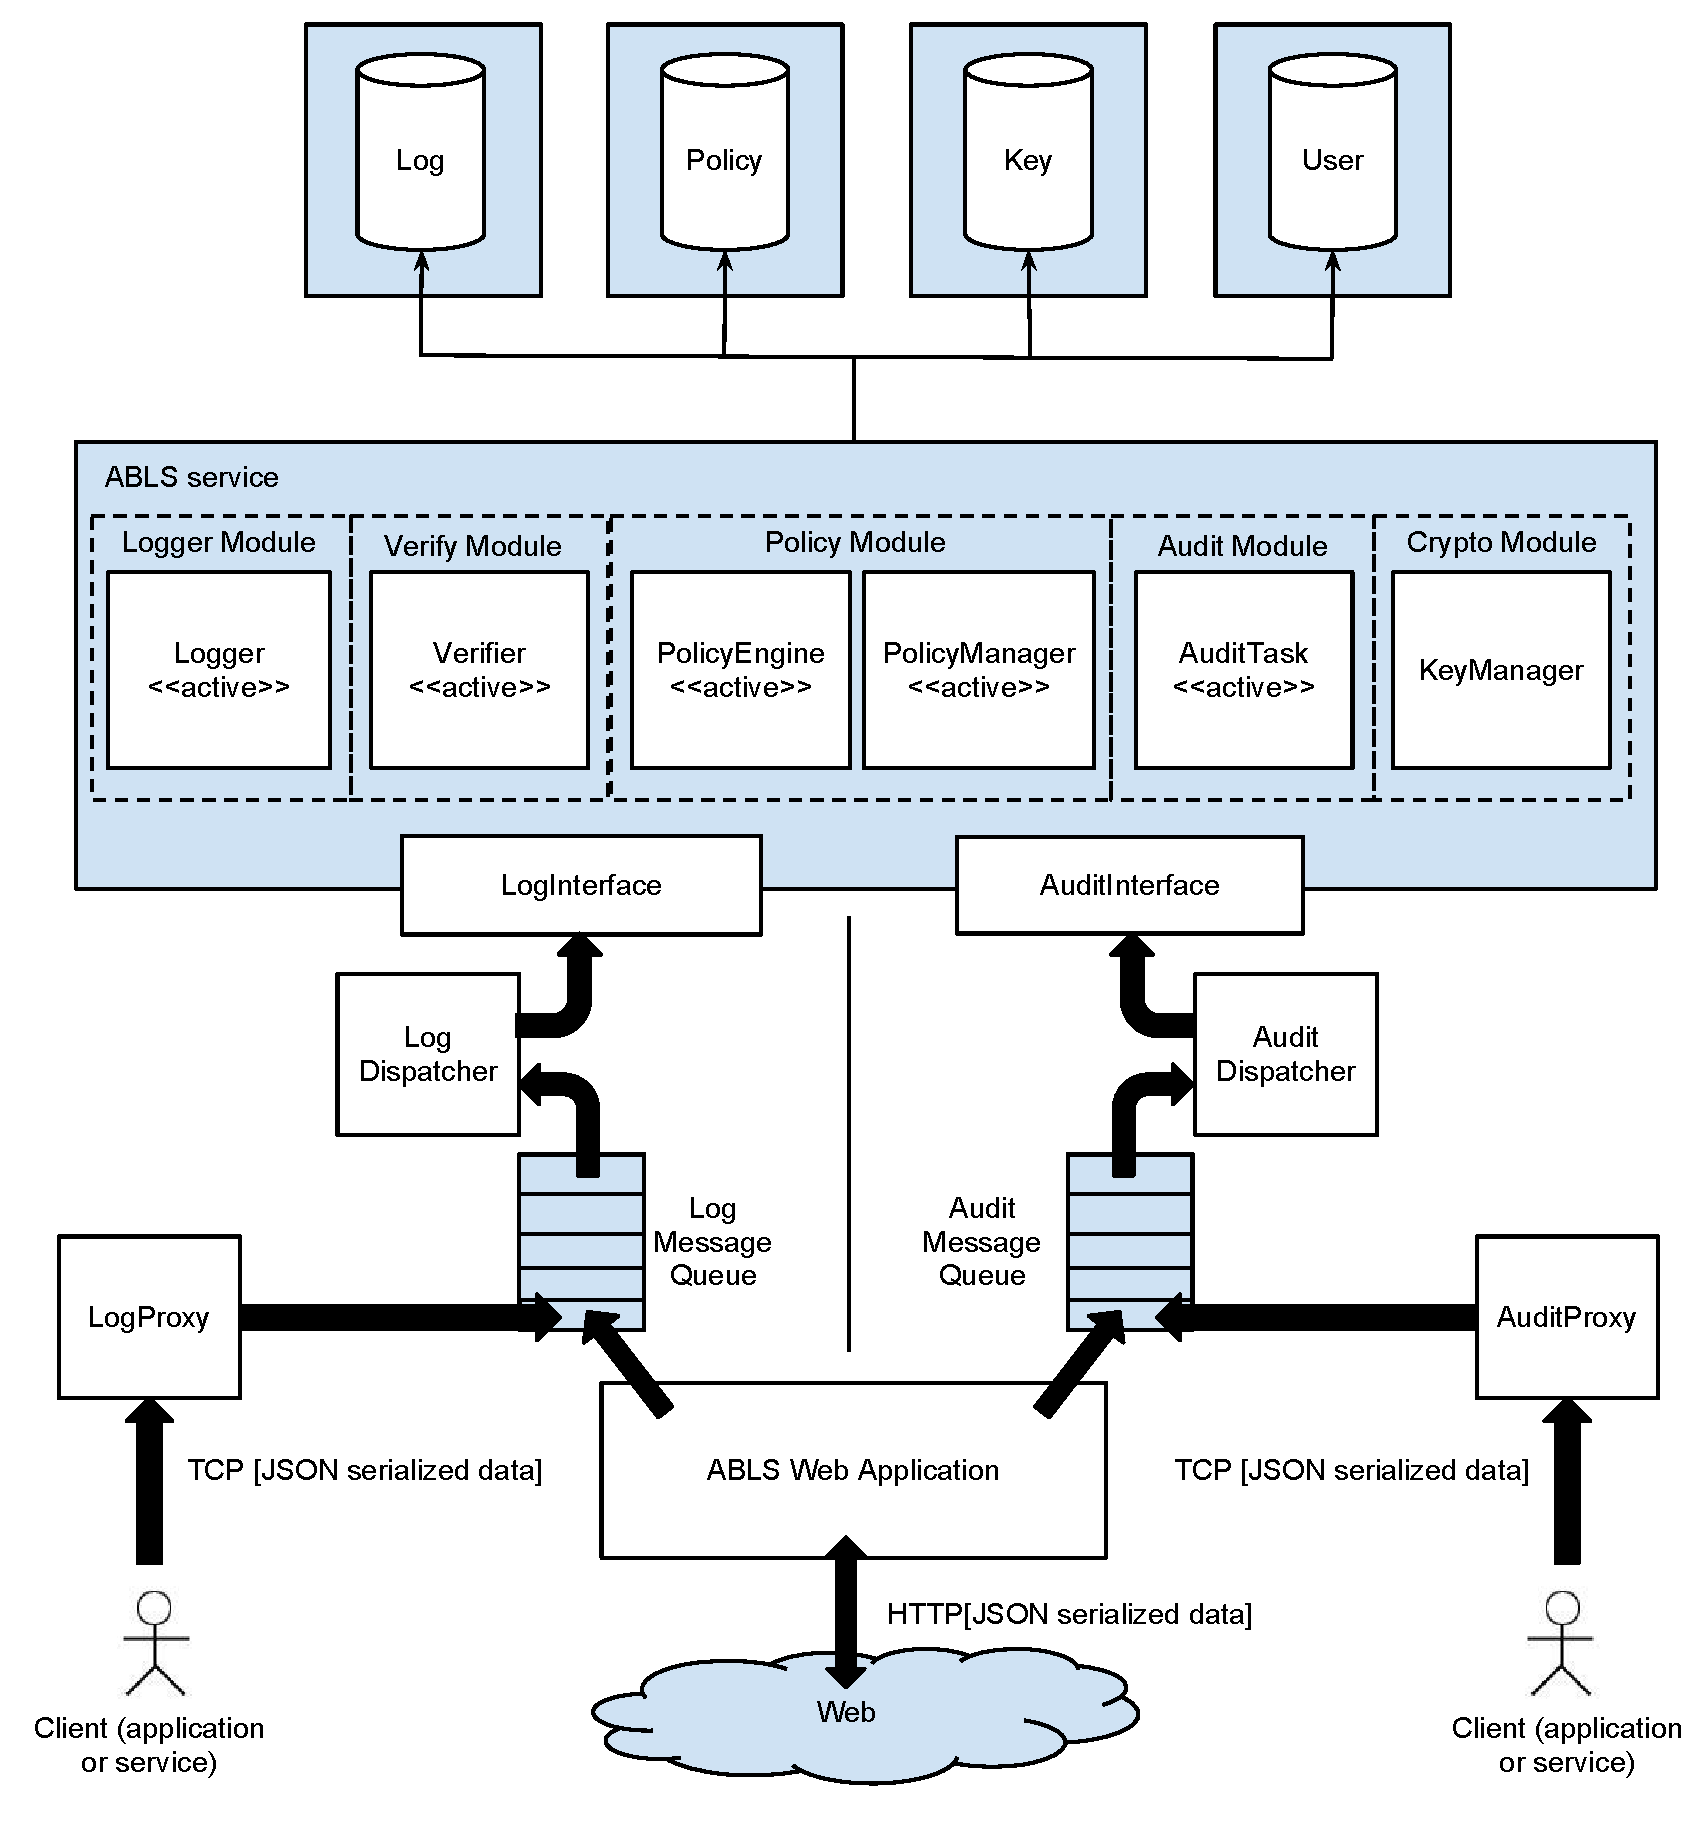
\includegraphics[width=5in]{images/deployment.pdf}
\caption{A high-level architectural diagram for ABLS. Message queues for log and audit data are used to separate the ABLS service from the front-end submission processes, thus enabling horizontal scalability if deployed the appropriate environment.}
\label{fig:deployment}
\end{center}
\end{figure*}

Based on the purpose of each piece of data used in the log, it is best to physically separate databases
that store data of different security classes rather than rely on a single, segregated database that uses MAC with 
polyinstantiation to protect data of different security classes. Of course, access control
and authentication mechanisms for all of the database servers is to be enforced at the operating system level, thus
prohibiting immediate access to all unauthorized users other than the internal tasks (i.e. logger, verifier, policy engine, etc) 
within an ABLS instance. 

\section{Performance Analysis}
The prototype ABLS system was written in Python, utilizing the Charm cryptography package 
\cite{akinyelecharm} for pairing-based cryptographic primitives. Since a major concern for the ABLS architecture 
was its scalable performance while processing large amounts of log data, we conducted experiments
to measure the encryption overhead from events that have uniform access policies, as well as the
encryption overhead from events that have different access policies. These two experiments were conducted to
guage the overhead of that results from log encryption and querying the policy engine for generating new policies.
The results for these two experiments are shown in Figures \ref{fig:logPerf} and \ref{fig:logPerfDiffEvents}. Based
on the resulting data, it was shown that a single log message requires approximately 180ms and 190ms to encrypt
if the data uses a pre-cached and newly-generated encryption key. Therefore, we conclude that the encryption
procedure has a more significant impact on the ABLS performance than the presence of the policy engine does. 
This is an indication that future optimizations would yield significantly better performance metrics.

\begin{figure}[ht!]
\begin{center}
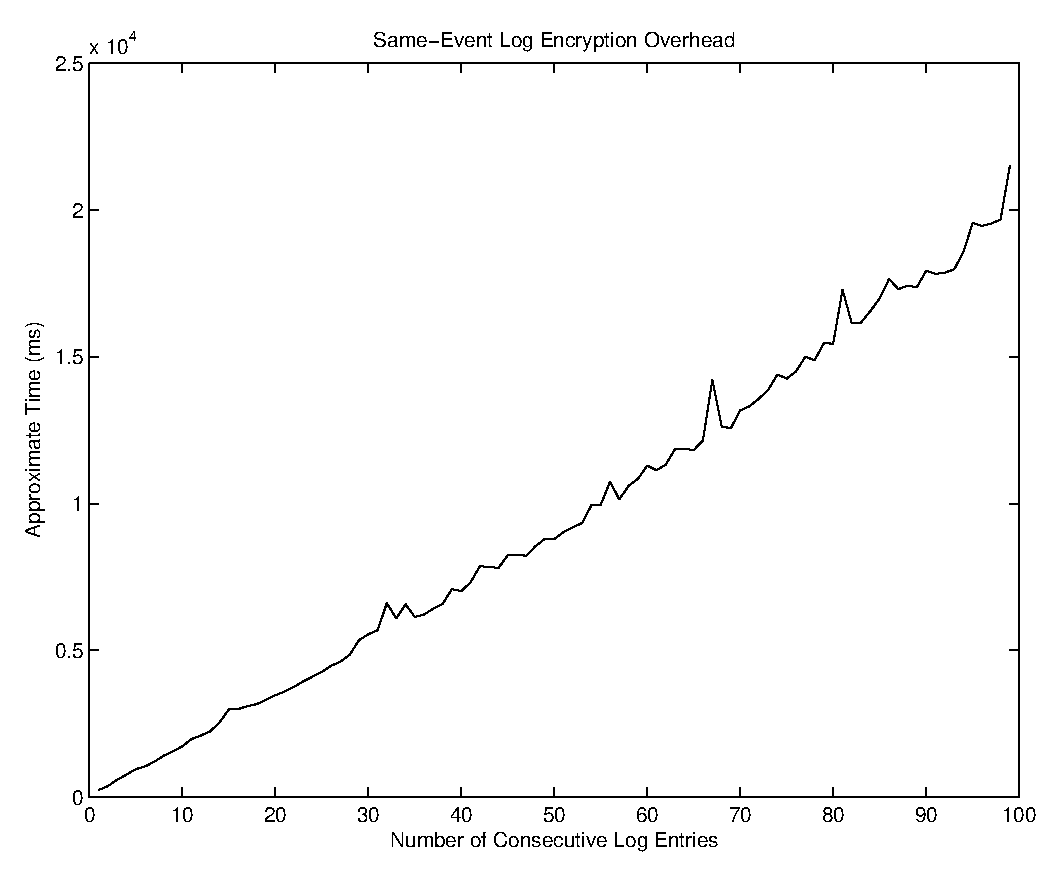
\includegraphics[width=3in]{images/logPerf.eps}
\caption{Log encryption performance for data in a single user session that all have the same access policy.}
\label{fig:logPerf}
\end{center}
\end{figure}

\begin{figure}[ht!]
\begin{center}
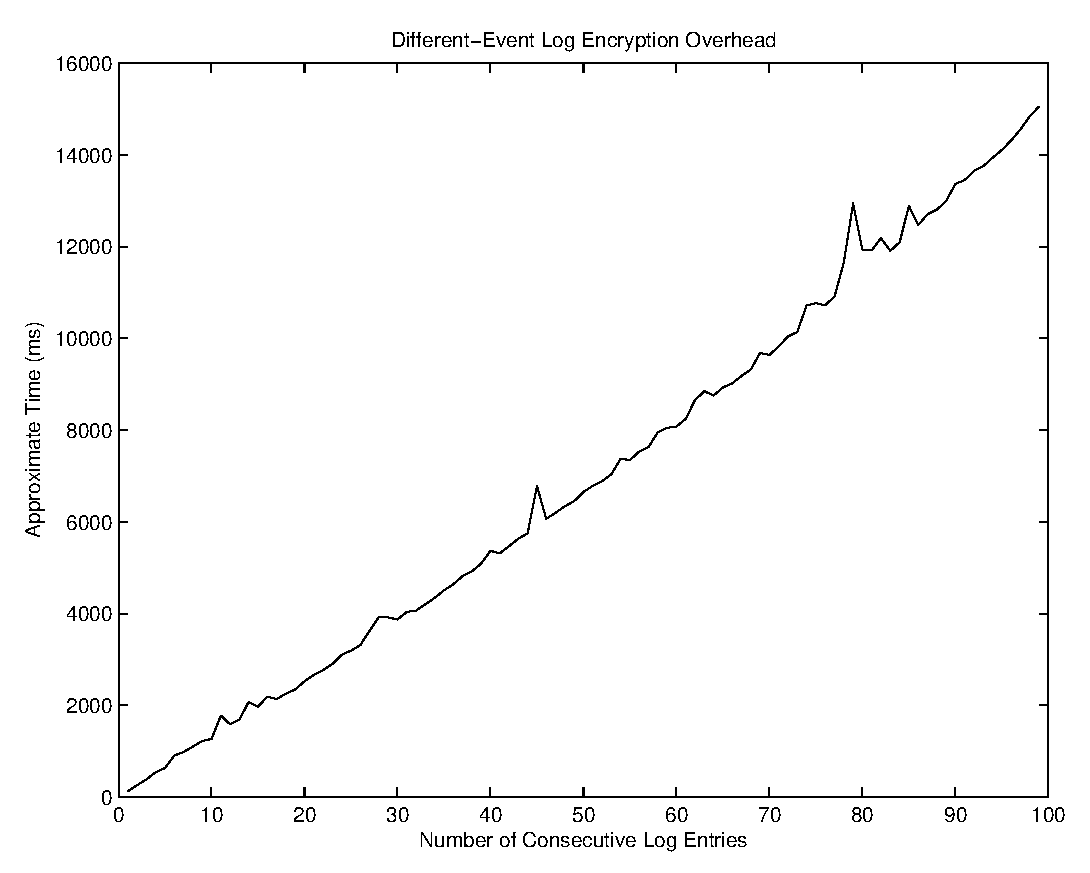
\includegraphics[width=3in]{images/logPerfDiffEvents.eps}
\caption{Log encryption performance for data in a single user session that all have different access policies.}
\label{fig:logPerfDiffEvents}
\end{center}
\end{figure}

To measure the storage overhead for the log data we compared the physical size of an empty SQLite database against
one that contained log data for three different policies, each with different numbers of attributes. The results of
this comparison are shown in Table \ref{tab:storage}. Based on this analysis, we concluded that each log entry contributed
approximately 1.2Kb of information to the log database, which is largely due to the highly conservative data types in the relational model.
This overhead could be drastically reduced if the model was adjusted to match the cryptographic primitives used in
the logging scheme and the use of BLOB attribute types was removed.

\begin{table}
\caption{Storage overhead for storing the log data}
  \begin{tabular}{|l|l|}
    \hline
    Log Database Contents & Storage Size (Kb) \\ \hline
    None & 12 \\ 
    100 log entries - minimal attributes & 134 \\ 
    100 log entries - medium attributes & 147 \\ 
    100 log entries - maximum attributes & 149 \\
    \hline
  \end{tabular}
  \label{tab:storage}
\end{table}

\section{Applications}
ABLS would be particularly useful in the healthcare domain, where organizations are required to comply with HIPAA 
policies and regulations \cite{king2012modifying}. Non-repudiation is a critical element that is 
needed to support these compliance efforts. Therefore,
configuring ABLS for use in these organizations can aid in the secure collection and persistence of relevant log information,
and also help automate the auditing process to reinforce the manual efforts done by security administrators. 

In such an environment, healthcare web applications would be configured to send all relevant user events to an ABLS 
instance in the cloud via the system HTTP API. All clients could be authenticated using a standard password-based 
scheme that is connected to the organization's user database. Similarly, all dedicated health machines and terminals in 
hospitals and physician offices would utilize continuous 
data streams to an ABLS instance and send all log data over a TCP socket using an API similar to that which is exposed to
web applications. These dedicated entities could be authenticated using two-way SSL authentication so 
as to allow authentication to take place using administrator-installed SSL certificates.

Security administrators could review the organization's required security policies and encode them using the popular 
XACML, which could be used to configure the ABLS policy engine for encrypting all incoming log data.
Similarly, the security administrators could define automated audit tasks that ensure policy violations do not occur. The 
security administrator would also be responsible for configuring the frequency at which automated audit and verification 
tasks and run. 

Although the current ABLS prototype does not currently export policy violations to a dashboard of any kind, in the event that 
this feature was added, the security administrator would also be responsible for configuring the connection between ABLS 
and the dashboard. Finally, depending on the rate at which the ABLS databases grow, the security administrator should 
also specify the parameters for archiving all audit data in a remote location. 

Once the overhead of configuring the ABLS instance for use with the organization's applications and dedicated machines,
the system enters a near autonomous state in which the administrator is only responsible for updating access policies 
for log data, modifying audit tasks (if needed), and manually inspecting policy violations when needed.

\section{Implementation Status}
The current ABLS implementation status is mostly up-to-date with the design and architecture presented 
in the preceding sections. We indicate notable features which were either needed to support some of the major design 
and architectural decisions for ABLS, or entirely orthogonal to these design decisions, in the following sections. It is
also important to note that there are three versions of ABLS: ABLS-V1, ABLS-V2, and ABLS-Main. Each of the following
sections are tagged with the corresponding ABLS version they refer to. All versions are included for the sake of 
completeness.

\subsection{[ABLS-Main] Web Application Front-End}
Although there was not much time to continue development during the final leg of this project, we were able to 
make a skeleton for the web application front-end using the Flask Python framework \cite{flask}. The web application
was configured to use the Flask security plugin to manage user session information and support the synchronization of  
information with the back-end ABLS service. Unfortunately, the connection to the back-end user database was not 
configured as part of this release due to a lack of time to finish this feature.

RabbitMQ \cite{rabbitmq}, a
distributed message queue based on the emerging AMPQ standard, was configured to tie the front-end to the 
back-end ABLS service. Although the functionality was not implemented to enable users to submit log data, log queries,
or audit tasks using the front-end, the messaging infrastructure and required architecture is currently implemented in order 
to support these features. There was simply not enough time to finish this task. 

\subsection{[ABLS-V1] Log Querying}
\label{sec:querying}
In order to make ABLS fulfill its purpose as a secure logging system, log query support through the audit
module is supported. Such query support is exposed to clients through a lightweight API that is used via the audit protocol.
Currently, only select operations parameterized by the user ID or both the user and session IDs are supported. 
The current version of the API has the following function signatures. \\

\noindent {\tt selectByUser(int uid)} \\
{\tt selectByUserAndSession(int uid, int sid)}\\

To use this API, clients connect to the audit proxy over a TCP socket, which is similar to the log traffic proxy initialization 
procedure, and issue commands according to the audit protocol to invoke either one of these functions. Once the client is 
authenticated, they can issue commands to the audit proxy as JSON strings with the following format. \\

\begin{lstlisting}
{     
    "command" : command_id
    "params" : csv_list
}
\end{lstlisting}

Upon receiving and parsing an incoming command, the client handler, which is spawned to handle each client connection,
issues the appropriate command to the log module to select log message contents from the database. 
A visual depiction of this protocol in action is shown in Figure \ref{fig:protocol}.

\begin{figure}[ht!]
\begin{center}
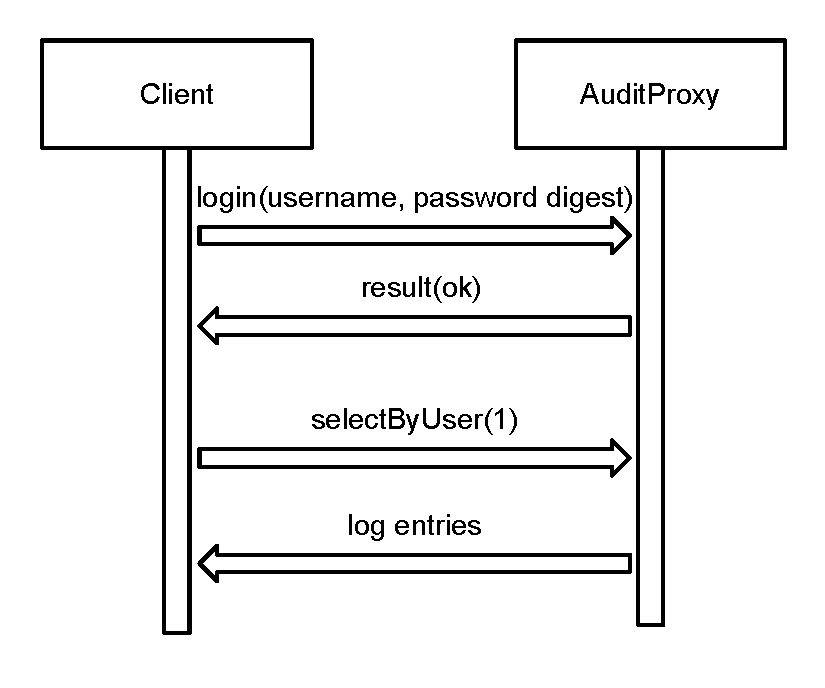
\includegraphics[width=3in]{images/logProtocol.pdf}
\caption{A simplistic sequence diagram of the log protocol, which is highly motivated by the popular FTP protocol.}
\label{fig:protocol}
\end{center}
\end{figure}

Unlike the log proxy, clients for the audit proxy are authenticated using user-defined passwords. Thus, as a
part of supporting client authentication, a proper password storage scheme was implemented in which the hash of 
password digests salted by a random string are persisted into the database. In this way, the user password is never sent 
in plaintext over the network. Also, the salt is stored in plaintext in the same audit\_user record, which is a common
practice for web applications.

\subsection{[ABLS-V1] Log Collection}
As part of the proposed design, all log messages generated by the logger to be inserted into the log
database were to be handed off to a common log collector to do so. This log collector is implemented as a 
separate thread running within the ABLS process and was designed to assume a portion of the database 
communication overhead from loggers to free up cycles for processing more log messages. Each logger instance
points to the same log collector thread. Furthermore, the log collector task is spawned when the ABLS 
instance first loads. Unfortunately, initial performance tests showed that the log collector was consuming too
many CPU cycles from other logger threads, and thus was removed from use in this version of ABLS. 
Future design enhancements may convert the log collector singleton into a log collection service backed 
by a pool of worker threads to handle database activity. 

\subsection{[ABLS-V1/V2] Bootstrapping, Test Enhancement, and Deployment}
In order to streamline the test and deployment phases of development for ABLS, a bootstrap script is provided to configure
new (empty) versions of the local SQLite databases. A different bootstrap Python script {\tt Bootstrap.py} is provided 
to clear the contents of every database and insert false user data into the users table. 
A test driver program, \\{\tt LogProxyDriver.py}, uses the now default data contained within the 
database. With these scripts and programs, the typical process to start and interact with an ABLS instance is as follows.

\begin{enumerate}
	\item Run the bootstrap script to create new versions of the local SQLite databases. In the actual deployment of an ABLS instance, this script would connect to the remote databases and specify their schemas accordingly. Thus, it is meant only for development purposes and should not be used on a live ABLS instance.
	\item Run {\tt Bootstrap.py} to insert fake data into the user database table.
	\item Run the main executable file ({\tt Main.py}) with the -l (log) flag to enable the logging service.	
	\item Run the test driver program ({\tt LogProxyDriver.py}) and point it to the host and port at which the log proxy within the ABLS instance is listening. By default, these are ``localhost'' and port 9998, but they can easily be changed to any other values in the ABLS configuration file. 
\end{enumerate}

Aside from the initialization code, the test driver program includes a robust suite of tests to simulate varying traffic 
loads. The user interface of this program was also improved so as to aid the developers in interacting with the ABLS 
prototype at runtime. Given the difficulty of testing this distributed system at runtime, creating a more sophisticated
test driver was crucial to the development process that enabled smoke tests to be run with minimal effort.

However, despite the complexity of the test driver, it does not, nor will it ever, support the ability to acquire 
diagnostic information from the ABLS runtime. This information is logged by the ABLS instances to the appropriate log 
file, and the administrators for the ABLS system can check this information at their discretion.

\subsection{[ABLS-V1/V2/Main] ABLS Configuration File} 
In order to improve the quality of the ABLS prototype, all of the hard-coded configuration strings that set up databases and 
network settings are placed in a configuration file ({\tt abls.conf}) that is managed by system administrators.
Access to this file can be restricted to system administrators and enforced by the 
operating system. An example of the configuration file is shown below.

\begin{lstlisting}
# Network configuration paramters
abls_host = localhost
abls_logger_port = 9998
abls_audit_port = 9999

# Database configuration string
location.db.log = ~/log.db
location.db.key = ~/key.db
location.db.users = ~/users.db
location.db.audit_users = ~/audit_users.db
location.db.policy = ~/policy.db
\end{lstlisting}

\subsection{[ABLS-V2] Automated Audit Support}
In the current system implementation, the log data model is configured according to the schema presented in
Section \ref{sec:model}. The proof-of-concept implementation for audit tasks enables a single audit task to be
spawned when the system is loaded that is responsible for enforcing policies specified by the LAudit language.
These audit tasks enforce audit rules using a blacklist approach, and are configured using audit task payloads
of the following form:

\begin{lstlisting}
[
    {
        role : "SuperUser",
        action : "Modified",
        object : "Object-X",
        affectedUsers : [1, 2, 3]
    }
]
\end{lstlisting}

Notice that the user attribute is replaced with a more abstract role attribute. Since it is rare that audit policies will
be specified at the level of individual users, this enables ABLS to enforce more generic audit rules across the 
entire database. If an audit task was given this rule definition, it would query the Event table for all
"Modified" actions performed on objects of type "Object-X" and join the results with the events in the AffectedUserGroup
table. With this data, it would check to see if any of the resulting records have affected users 1, 2, or 3 in them, and if
so, generate an error or alarm. 

The current implementation supports the new log and event chaining, log message parsing, and 
audit task configuration using the techniques described throughout this paper. However, the code is mostly a 
proof-of-concept implementation, and is not integrated into the entire ABLS system architecture. That is, test-code is 
embedded in the {\tt Chainer.py} and {\tt Auditor.py} files to demonstrate that this new automated audit technique works as 
expected.

\section{Lessons Learned}
This project was extremely educational. Perhaps the most important lesson from that we took away from this work
was that cryptography is not a one-time solution to every problem. In the case of secure logging systems, there
is a plethora of other factors that must be considered for the system to be \emph{secure, correct, and efficient}. 
Furthermore, achieving automated audits in a secure logging system is a non-trivial challenge that must strike a 
balance between system performance and storage overhead, as indicated by our performance results. 

Another important less that we took away from this work is that ambiguity in security policy definitions and log
data structure makes automated auditing an incredibly challenging task. If there is no standard by which log 
data will be sent to the logging system, or by which security policies will be defined, then, quite simply, there cannot 
be an efficient programmatic solution for comparing policies against log data. 

Another key aspect from this project was that key management is a difficult problem to solve in any context, especially
when a variety of cryptographic primitives are in use (i.e. CP-ABE, symmetric-key AES, and keyed MACs). The security
of encrypted data cannot be guaranteed without an appropriate mechanism for storing and protecting these keys, which
therefore means that key management is a fundamental problem to solve for secure logging systems. We also learned
that mixing cryptographic primitives (i.e. using CP-ABE to encrypt symmetric keys that encrypt log data) can pay 
performance dividends without sacrificing security. Therefore, the application of cryptographic primitives must be
carefully considered from both a security and performance perspective. 

Finally, we learned that supporting automated audits through the LAudit language introduces a great deal of overhead. 
This was an expected result due to the amount of extra information that was created and stored for each log entry,
but the benefit was that it enabled us to leverage SQL to efficiently query the database for policy violations. This 
implies that there is always a space and time tradeoff when designing complex software solutions to seemingly simple 
problems.

\section{Future Work}
While the current ABLS design provides efficient automated audits to help support non-repudiation, 
there are several fundamental design changes that can be explored for further improvement. One such change 
is the application of publicly-verifiable FssAgg signature generation algorithms to generate entity tags for log chains. 
This would reduce the storage overhead for log information by ultimately removing the need to use hash chains
altogether and reduce the signature generation (aggregation) time without sacrificing the complexity of signature
verification. However, these schemes require a trusted CA for public verification, which may or may not be available
in the environments where ABLS would be deployed. 

Another avenue for future work is the removal of the online server dependence for log verification and temporal
(time-sensitive) log decryption. The author does not know how this design problem would be solved, but it is worth
investigating in the future. 

Finally, the LAudit language should be expanded to include more temporal information in the grammar, such as 
time ranges where a policy might be in effect. For example, it should be possible to specify a time of day where access
to a certain object by a certain type of user is prohibited. The current grammar does not support this capability. 

\section{Conclusion}
In this paper we presented ABLS, a secure logging system for the cloud that supports automated audits and
attribute-based log file encryption. We discussed the log integrity and confidentiality properties supported by ABLS, 
and how they map to the underlying system architecture and relational data model. We then presented the current
architecture and deployment scheme for an ABLS instance in the cloud, which included the client interfaces for 
submitting log data and executing audit queries. We finished with a performance analysis of the current ABLS prototype 
and discussion of employing ABLS in the healthcare domain. 

\begin{comment}
\begin{table}
\centering
\caption{Feelings about Issues}
\begin{tabular}{|l|r|l|} \hline
Flavor&Percentage&Comments\\ \hline
Issue 1 &  10\% & Loved it a lot\\ \hline
Issue 2 &  20\% & Disliked it immensely\\ \hline
Issue 3 &  30\% & Didn't care one bit\\ \hline
Issue 4 &  40\% & Duh?\\ \hline
\end{tabular}
\end{table}

\begin{figure}[htb]
\label{sample graphic}
\begin{center}
\includegraphics[width=1.5in]{fly.jpg}
\caption{A sample black \& white graphic (JPG).}
\end{center}
\end{figure}
\end{comment}

\bibliographystyle{abbrv}
\bibliography{../abls}
% You must have a proper ".bib" file
%  and remember to run:
% latex bibtex latex latex
% to resolve all references
\balance
\end{document}
